\documentclass[11pt]{scrartcl}
\usepackage{dominatrix}
\usepackage{solarized-light}
\lstset{
language=R
}

\newcommand{\sgn}{\ensuremath{\mathrm{sgn}}}

\usepackage{dsfont}

\title{Homework 2}
\subject{Statistical Machine Learning (STAT W4400)}
\author{Linan Qiu\\\texttt{lq2137}}
\begin{document}
\maketitle

\textbf{As usual, code is available at \url{https://github.com/linanqiu/stat-w4400-homework}}

\section{Adaboost}

\subsection{Implement Adaboost in R}

Done in \texttt{adaboost.R}

\subsection{Implement decision stump \texttt{train} and \texttt{classify}}

Done in \texttt{stump.R}

To generate weak learners, I guessed a $\theta$, then if the $\theta$ produces a cost greater than 5, I took the negative $m$.

\subsection{Run Algorithm on USPS Data}

Done in \texttt{adaboost.R} with $K$ crossfold validation (defaults to 5).

\subsection{Plot Training and Testing Error}

Plots shown next page.

\begin{landscape}
\begin{figure}[H]
\centering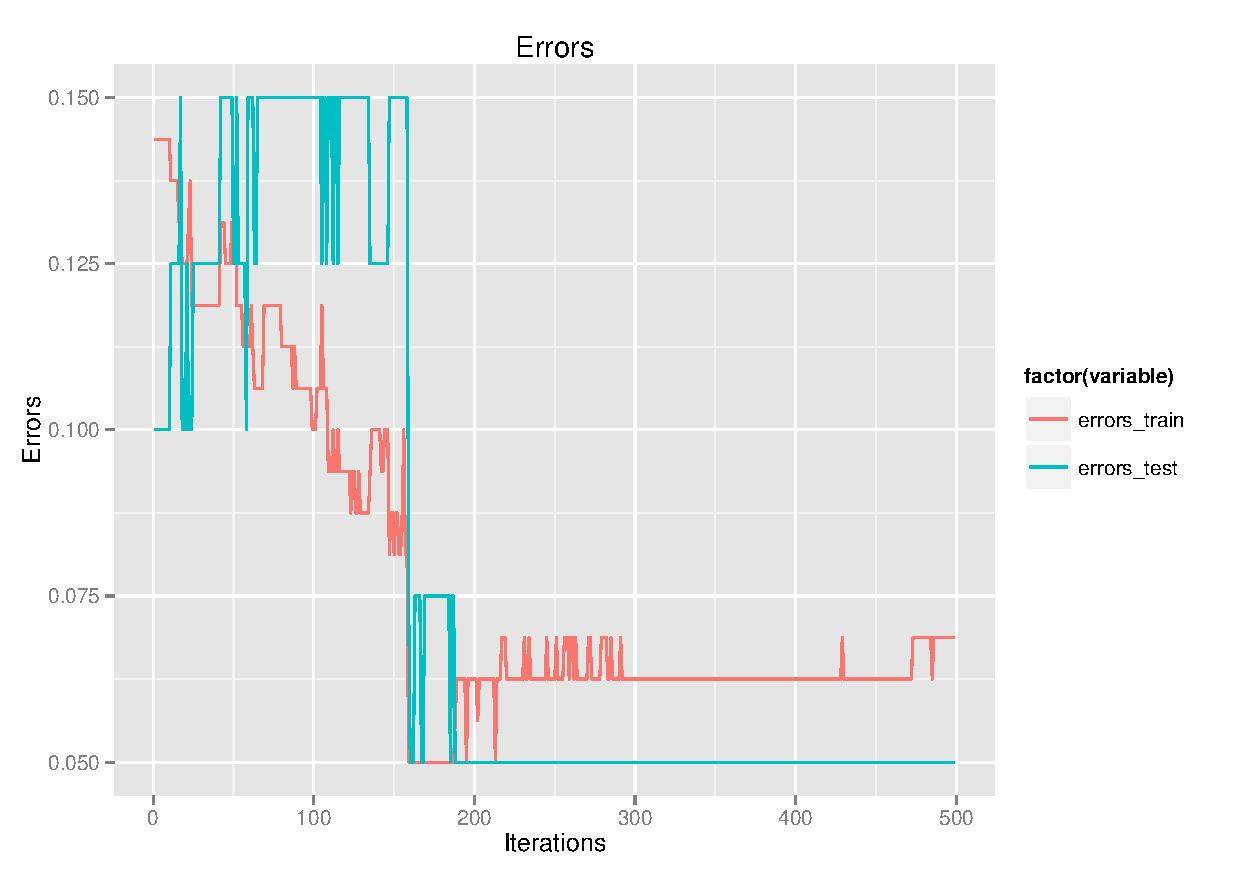
\includegraphics[width=\textwidth]{./hw3/adaboost-500.pdf}
\caption{Except for a weird spike in test error after around 100 iterations (probably due to the weak nature of the learners) we see a rather fast decrease in test error.}
\end{figure}

\begin{figure}[H]
\centering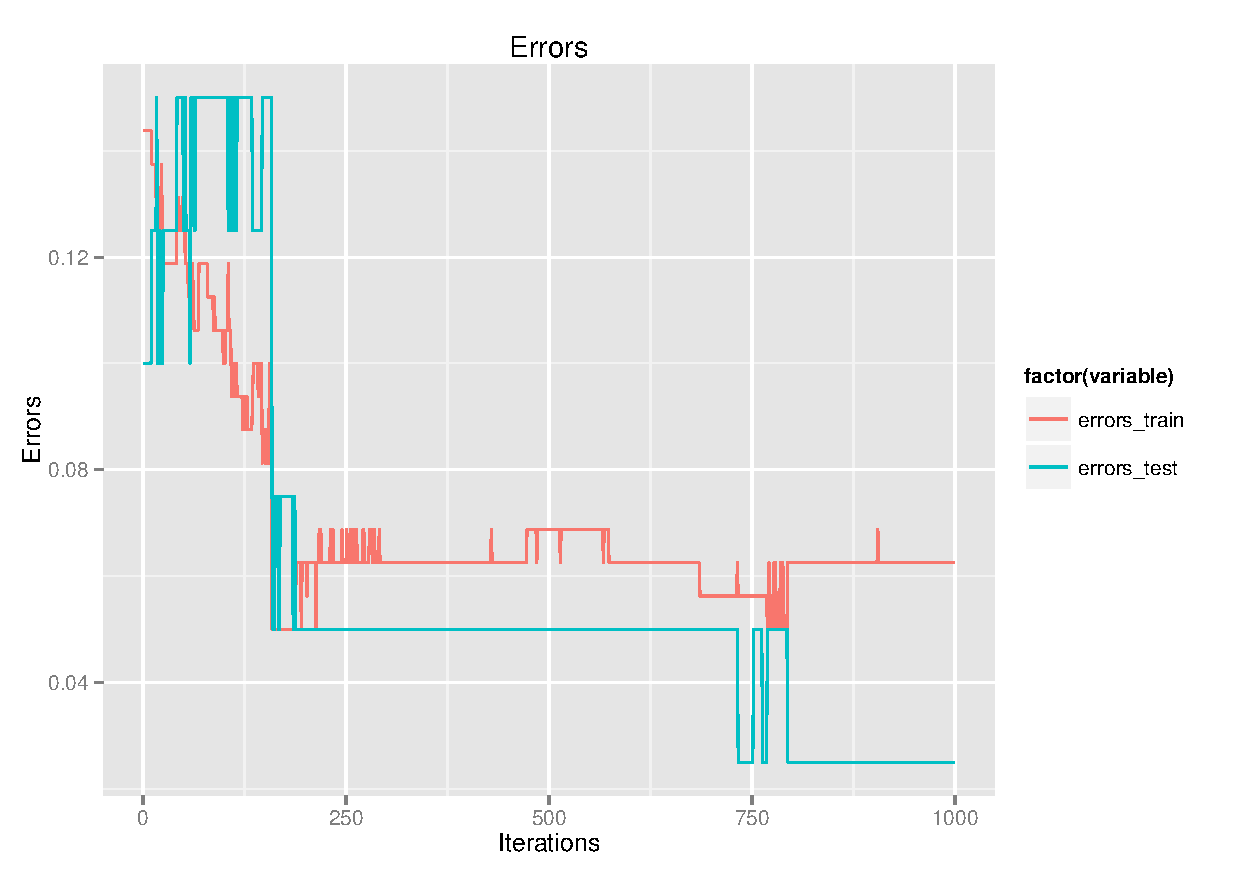
\includegraphics[width=\textwidth]{./hw3/adaboost-1000.pdf}
\caption{The decrease continues into 1000. However, the quantized nature of the jumps (due to the small data size) is not helpful at all.}
\end{figure}
\end{landscape}

\section{}

\subsection{}

The left cost function encourages sparse estimates. It prefers points in $\hat{\beta}$ that have either $\beta_1$ or $\beta_2$ but not both, whereas the one on the right tends to encourage the opposite. This is already evident in the illustration, where $x_3$ and $x_5$ intersects with $\hat{\beta}$.

\subsection{}

\begin{itemize}
\item For $q=0.5$, $x_3$ minimizes the cost as it is the only point to intersect the constraint region.
\item For $q=4$, $x_3$ and $x_5$ intersects, but $x_4$ minimizes the cost since it lies within the constraint region, and would be lower cost than $x_3$ and $x_5$ that satisfies the constraint but lie on the border.
\end{itemize}

\end{document}
